\documentclass[12pt, letterpaper]{article}
\usepackage[hyphens]{url}
\setlength{\topmargin}{-1.75cm} \setlength{\textheight}{22.5cm}
\setlength{\oddsidemargin}{0.25cm}
\setlength{\evensidemargin}{0.25cm} \setlength{\textwidth}{16.2cm}
\renewcommand{\figurename}{Figure}
\usepackage{amssymb}
\usepackage{graphicx}
\usepackage{amsmath}
\usepackage[normalem]{ulem}
\usepackage{fontenc}
\usepackage{footnote}
\usepackage[breaklinks]{hyperref}
\usepackage{palatino, multicol, listings} % for multiple columns
\lstset{mathescape=true, basicstyle=\ttfamily,}

%\usepackage{pictex}
%% in the .pictex output of xfig, there is command \colo
%% however the old version of pictex may not define this
%% so we define color here as empty
%\def \color#1]#2{}

\begin{document}

\newcommand{\hide}[1]{}
\newcommand{\exercise}[1]{}
\newcommand{\future}[1]{}
\newcommand{\otherquestions}[1]{}
\newcommand{\set}[1]{\{#1\}}
\newcommand{\pg}[1]{{\tt #1}}
\newtheorem{definition}{Definition}
\newcommand{\emptyclause}{\Box}
\def\st{\bigskip\noindent}
\newcommand{\lplus}
{
   \stackrel{+}{\gets}
}

\newcommand{\fe}[1] {
  \begin{frame}
    #1
  \end{frame}}

\newcommand{\eoa}{ {\bf End} of algorithm}

\newcommand{\ft}[1] {\frametitle{#1}}

\newcommand{\ie}[1] {
  \begin{itemize}
    #1
  \end{itemize}
}

\newcommand{\ee}[1] {
  \begin{enumerate}
    #1
  \end{enumerate}\label{marker}
}
\newcommand{\blk}[2] {
  \begin{block}{#1}
    #2
  \end{block}
}

\newtheorem{collorary}{Corollary}
\newtheorem{proposition}{Proposition}
\newtheorem{invariant}{Invariant}
\newtheorem{property}{Property}
\newtheorem{claim}{Claim}
\newtheorem{example}{Example}


\title{${\cal ELPS}$ manual}
\date{\today}
\maketitle
\tableofcontents
\pagebreak


\section{System installation}

\st For using the system, you need to have the following installed:
\begin{enumerate}
\item Java Runtime Environment (JRE): \\
{\scriptsize
\url{http://www.oracle.com/technetwork/java/javase/downloads/index.html}
}.\\
The system was tested on Java versions 1.6.0\_37 and 1.7.0\_25.
\item The ELPS binary file: \\ 
{\scriptsize
\url{https://github.com/iensen/elps/blob/master/elps.jar?raw=true}
}.

\item Clingo (version 4.2.1 or later):\\ {\scriptsize
 \url{http://sourceforge.net/projects/potassco/files/clingo/4.2.1}}


\end{enumerate}

Be sure the PATH system variable includes the directory where the clingo executable is located. For instructions on how to view/modify the PATH system variable, see either of the following links:\\
{\scriptsize
\url{http://www.java.com/en/download/help/path.xml}\\
\url{http://www.cyberciti.biz/faq/appleosx-bash-unix-change-set-path-environment-variable/}\\
}
To check if the solver is installed correctly, run the command  \texttt{clingo - v}. See figure \ref{fig:clingo_solver_check} for the expected output.

\begin{figure}[h!]
\centering
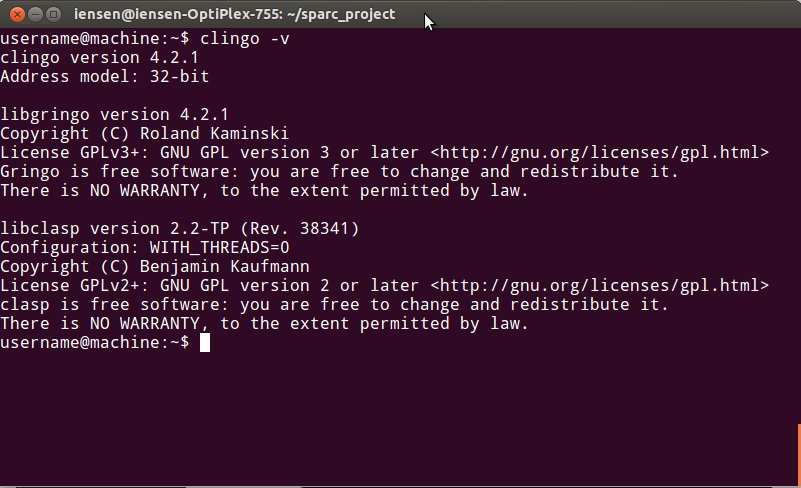
\includegraphics[width=0.9\textwidth]{clingo_version.jpg}
\caption{Checking the version of Clingo solver}
\label{fig:clingo_solver_check}
\end{figure}

\section{System usage}

To demonstrate the usage of the system we will use the program $\Pi$ below described in \cite{epist}.
\begin{verbatim}
sorts
#student = {mike,mary,ann}.

predicates

eligible(#student).
highGPA(#student).
fairGPA(#student).
minority(#student).
interview(#student).

rules
eligible(X):- highGPA(X).
eligible(X):- minority(X), fairGPA(X).
-eligible(X):- -fairGPA(X), -highGPA(X).
interview(X):- not K$ eligible(X), not K$ -eligible(X).

% data
fairGPA(mike) | highGPA(mike).
highGPA(mary).
\end{verbatim}

To run  ${\cal ELPS}$ solver  on the program above, 
we change current directory to a directory having the file \texttt{program.sp} with the program written in it, and the downloaded file \texttt{elps.jar}.  Then, we run the command:
\begin{verbatim}
iensen@iensen-OptiPlex-755:~/elps$ java -jar elps.jar elib.lp
ELPS V1.02
program translated
World View 1 out of 1
{{eligible(mary), student(mary), student(mike), interview(mike),
 highGPA(mary), fairGPA(mike)}, {eligible(mary), student(mary),
 student(mike), interview(mike), highGPA(mike), highGPA(mary),
 eligible(mike)}}

\end{verbatim}
The program has a single world view, which contains \texttt{interview(mike)} in both believe sets.




\section{Syntax Description}

\subsection{Directives}
Directives should be written before sort definitions, at the very beginning of a program.
${\cal ELPS}$ allows two types of directives:
\subsection*{\#maxint}
Directive \#maxint specifies maximal nonnegative number which could be used in arithmetic calculations. For example,
\begin{verbatim}
 #maxint=15.
\end{verbatim}
\st limits integers to [0,15].
\subsection*{\#const}
Directive \#const allows one to define constant values. The syntax is:

\begin{verbatim}
   #const constantName = constantValue.
\end{verbatim}      
\st where $constantName$  must begin with a lowercase letter and may be composed of letters, underscores and digits,
 and $constantValue$ is either a nonnegative number or the name of another constant defined above.  


\subsection{Sort definitions}\label{ss}

This section starts with a keyword $sorts$ followed by a collection of sort definitions of the form:

\begin{verbatim}
  sort_name=sort_expression.
\end{verbatim}
\texttt{sort\_name} is an identifier preceeded by a pound sign \#.
\texttt{sort\_expression}  on the right hand side denotes collection of strings called $sorts$. We divide all the sorts into \textit{basic} and \textit{non-basic}. 

\st \textit{Basic sorts} are defined as named collections of identifiers, i.e, strings consisting of
\begin{itemize}
 \item latin letters: $\{a,b,c,d,...,z,A,B,C,D,...,Z\}$
 \item digits: $\{0,1,2,...,9\}$
 \item underscore: $\_$
\end{itemize}
and either starting from a letter or containing only digits.

Non-basic sorts also contain \textit{records} of the form $id(\alpha_1,\dots, \alpha_2)$, where id is an identifier and 
$\alpha_1, \dots, \alpha_n$ are either identifiers or records. 


\st We define sorts by means of expressions (in what follows sometimes referred as statements) of five types:

\begin{enumerate}

\item \textbf{numeric range}.
\begin{verbatim}
 numeric_range := number1..number2
\end{verbatim}

\textit{number1} should be smaller or equal than \textit{number2}. The expression defines the set 
of subsequent numbers $\{number1, number1+1, \dots, number2\}$

\textit{Example:}

\begin{verbatim}
 #sort1=1..3
\end{verbatim}
\texttt{\#sort1} consists of numbers $\{1,2,3\}$.


\item \textbf{identifier range}


\begin{verbatim}
 id_range := id1..id2
\end{verbatim}

\textit{id1} should be lexicographically smaller or equal than \textit{id2}. 
\textit{id1} and \textit{id2} should both consist of digits and letters and start from a lowercase letter.
The expression defines the set of all strings \\ S=$\{s: id1\leq s \leq id2 \land |id1|\leq |s| \leq |id2|\}$



\textit{Example:}

\begin{verbatim}
 #sort1=a..f.
\end{verbatim}

\texttt{\#sort1} consists of latin letters $\{a,b,c,d,e,f\}$.

\item \textbf{set of ground terms}


\begin{verbatim}
 ground_terms_set := {t_1,..,,t_n}
\end{verbatim}

\texttt{ground\_terms\_set} denotes a set of ground terms $\{t_1,...,t_n\}$, defined as follows:
\begin{itemize}
 \item numbers and constants are ground terms;
 \item If $f$ is an identifier and $\alpha_1, \dots, \alpha_n$ are ground terms, then $f(\alpha_1,\dots, \alpha_n)$ is a ground term.
\end{itemize}
\textit{Example} : 
\begin{verbatim}
 #sort1={f(a),a,b,2}.
\end{verbatim}






\item \textbf{record}


\begin{verbatim}
 functional_term := f(sort_name1(var_1),..., sort_namen(var_n)):
                                     condition(var_1,...,var_n)
 condition(var_1,...,var_n) := var_i REL var_j 
 condition(var_1,...,var_n) :=   condition and condition 
              | condition or condition 
              | not(condition) 
              | (condition)
\end{verbatim}
Variables \texttt{var\_1,...,var\_n} are optional as well as the condition.
Condition can only contain variables from the list \texttt{var\_1,...,var\_n}.
If there is a subcondition \texttt{var\_i REL var\_j}, where REL is either $\{>,\geq,<,\leq\}$ then \texttt{sortname\_i} and then \texttt{sortname\_j}
must be defined by basic statements.

The expression defines a collection of ground terms 
\\ $\{f(t_1,\dots,t_n): condition(t_1,\dots, t_n)~is~true \land t_1 \in s_i \land \dots \land t_n \in s_n\}$

\textit{Example}
\begin{verbatim}
 #s=1..2.
 #sf=f(s(X),s(Y),s(Z)): (X=Y or Y=Z). 
\end{verbatim}

The sort \texttt{\#sf} consists of records $\{f(1,1,2),f(1,1,1),f(2,1,1)\}$
 \item \textbf{set-theoretic expression}.
 \begin{verbatim}
  set_expression := sort_name | ground_term_set|functional_term
  set_expression := (set_expression) 
                    | (set_expression + set_expression ) 
                    | (set_expression * set_expression ) 
                    | (set_expression - set_expression )
  \end{verbatim}
\texttt{sort\_name} must be a name of a sort occurring in one of the preceeding sort definitions. 
The operations $+$ $*$ and $-$ stand for union, intersection and difference correspondingly.

\textit{Example} : 
\begin{verbatim}
 #sort1={a,b,2}.
 #sort2={1,2,3} + {a,b,f(c)} + f(#sort1).
\end{verbatim}
 \texttt{\#sort2} consists of ground terms $\{1,2,3,a,b,f(c),f(a),f(b),f(2)\}$.
\item \textbf{concatenation}
\begin{verbatim}
concatenation := [b_stmt_1] ... [b_stmt_n]
\end{verbatim}

\texttt{b\_stmt\_1}, $\dots$, \texttt{b\_stmt\_n} must be \textit{basic statements}, defined as follows:


\begin{itemize}
 \item statements of the forms (1)-(3) are basic
 \item statement $S$ of the form (5) is basic if:
 \begin{itemize}
 \item it does not contain sort expressions of the form (4), denoting sets of records
  \item all curly brackets occurring in $S$ contain only constants consisting of latin letters and digits
  \item all sorts occurring in $S$ are defined by basic statements 
 \end{itemize}
\end{itemize}
Note that basic statement can only define a basic sort not containing records.

\textit{Example\footnote{We allow a shorthand `b` for singleton  set \{b\}}.:}

\begin{verbatim}
 #sort1=[b][1..100].
\end{verbatim}

\texttt{sort1} consists of identifiers $\{b1,b2,\dots, b100\}$.

\end{enumerate}

\subsection{Predicate Declarations}

\noindent  The second part of a  ${\cal ELPS}$ program starts with the keyword
\st
$predicates$

\st and is followed by statements of the form

\st
$pred\_symbol(\#sortName,\dots,\#sortName)$

\st

Multiple declarations containing the same predicate symbol are not allowed.
0-arity predicates must be declared as $pred\_symbol()$.
\st For any sort name $SN$, the system includes declaration  $SN(SN)$ automatically.

\subsection{Program Rules}


\st The third part of a ${\cal SPARC}$ program starts with the keyword \textit{rules} followed by  rules of the form.

\begin{equation}
   \ell_0 | \ell_1 \dots |\ell_n \gets \ell_{n+1},  \ldots, \ell_{m}, not~\ell_{m+1} \ldots not~\ell_{k}
\end{equation}
where each $l_i$ is either a literal or a subjective literal. Subjective literals can be in one of the forms $K\$\ell$,$M\$\ell$, $not~ K\$\ell$, $not~M\$\ell$.
 
Literals occurring in the heads of the rules must not be formed by predicate symbols
occurring as sort names in sort definitions. In addition, rules must not contain \textit{unrestricted variables}.

\begin{definition}(Unrestricted Variable)
 A variable occurrung in a rule of a ${\cal SPARC}$ program is called unrestriced if all its occurrences in the rule either belong to some relational atoms of the form 
$term1$ \textbf{rel} $term2$ (where \textbf{rel} $\in  \{>,>=,<,<=,=,!=$\})  and/or  some terms appearing in a head of a choice or aggregate element. 
\end{definition}
\begin{example}
\em{
 Consider the following ${\cal ELPS}$ program:
\begin{verbatim}
sorts
#s={f(a),b}.
predicates
p(#s).
rules
p(f(X)):-Y<2,2=Z,F>3,#count{Q:Q<W,p(W),T<2},p(Y).
\end{verbatim}
Variables F,T,Z,Q are unrestricted.
}  
\end{example}

 

\section{Typechecking}
If no syntax errors, are found,  a static check program is performed all found type-related problems, classified into type errors and type errors.
\subsection{Type errors}
Type errors are considered as serious issues which make it  impossible to complied and execute the program.
Type errors can occur in all four section of a ${\cal SPARC}$ program.
\subsubsection{Sort definition errors}
\begin{enumerate}
\item  Set-theoretic expression (statement (2) in section \ref{ss}) contains a name of undefined sort.

\textit{Example:}
\begin{verbatim}
 sorts
 #s={a}.
 #s2=#s1-s.
\end{verbatim}

\item  Sort with the same name is defined more than once.
\textit{Example:}
\begin{verbatim}
 sorts
 #s={a}.
 #s={b}.
\end{verbatim}

\item In an identifier range id1.. id2 (statement (2) in section \ref{ss}) the first identifier(id1) is lexicographically greater than id2.
\textit{Example}
\begin{verbatim}
 sorts
 #s=zbc..cbz.
\end{verbatim}

\item In a numeric range $n1..n2$ (statement (2) in section \ref{ss})  n1 is greater than n2.
\textit{Example:}
\begin{verbatim}
 sorts
 #s=100500..1.
\end{verbatim}


\item Numeric range (statement (2) in section \ref{ss}) $n1..n2$  contains an undefined constant.

\begin{verbatim}
 #const n1=5.
 sorts
 #s=n1..n2.
\end{verbatim}

\item In an identifier range $id1..id2$ (statement (3) in section \ref{ss})  the length of the first identifier(id1) is greater than length of the second. 


\textit{Example:}
\begin{verbatim}
 sorts
 #s=abc..a.
\end{verbatim}

\item Concatenation (statement  (4) in section \ref{ss}) contains a non-basic sort.

\textit{Example:}
\begin{verbatim}
 sorts
 #s={f(a)}.
 #sc=[a][#s].
\end{verbatim}



\item Record definition (statement (5) in section \ref{ss}) contains an undefined sort.

\textit{Example:}
\begin{verbatim}
 sorts
 #s=1..2.
 #fs=f(s,s2).
\end{verbatim}



\item Definition of record (statement (5) in section \ref{ss}) contains a condition with relation $>,<,\geq,\leq$ such that the
   corresponding sorts are not basic.
\textit{Example:}
\begin{verbatim}
#s={a,b}.
#s1=f(#s). 
#s2=g(s1(X),s2(Y)):X>Y.
\end{verbatim}

\item  Variable is used more than once in record definition(statement  (5) in section \ref{ss}).

\textit{Example:}

\begin{verbatim}
 sorts
 #s1={a}.
 #s=f(#s1(X),#s1(X)):(X!=X).
\end{verbatim}
\item Sort contains an empty collection of ground terms.

\textit{Example}
\begin{verbatim}
 sorts
 #s1={a,b,c}
 #s=#s1-{a,b,c}.
\end{verbatim}
\end{enumerate}
\subsubsection{Predicate declarations errors}

\begin{enumerate}
\item A predicate with the same name is defined more than once.
\textit{Example:}
\begin{verbatim}
 sorts
 #s={a}.
 predicates
 p(#s).
 p(#s,#s).
\end{verbatim}
\item A predicate declaration contains an undefined sort.
\textit{Example:}
\begin{verbatim}
 sorts
 #s={a}.
 predicates
 p(#ss).
\end{verbatim}
\end{enumerate}
\subsubsection{Program rules errors}

In program rules we first check each atom of the form $p(t_1,\dots,t_n)$ and each term occurring in the program $\Pi$ for satisfying
the definitions of program atom and program term correspondingly\cite{sparc}. Moreover, we check that no sort occurs in a head of a rule of $\Pi$.

\bibliography{mybib}
\bibliographystyle{plain}
\end{document}

